\chapter{State of the Art}\label{StateOfTheArt}
In this chapter we will go over the latest improvements for CNNs. 
They range from the activation function used within each neuron to major architecture overhauls from the original LeNet-5.


\section{Recent Advances in Training Neural Networks}\label{s:NNAdvances}

\subsection{Activation Functions}
There have been many recent papers on improving the results of NNs in general. One focus has been on the activation functions used inside the network. The current trend has been using activation functions that are non-saturated, meaning they do not have very small derivatives at large input values. All mentioned activation functions can be seen in Fig.~\ref{f:activations}.

\paragraph{ReLU:}
The most notable non-saturated activation function is the rectified linear unit (ReLU) \cite{nair2010rectified}. This is defined as:
\begin{equation}
f(x) = \mbox{max}(0,x).
\label{e:relu}
\end{equation}
The benefits of this unit include: faster calculation since the max($\cdot$) operation is faster than sigmoid or tanh, it creates sparsity in the hidden units by giving true zero values often to help sparse representations form, and does not suffer from vanishing gradients in deep models. ReLU has been shown to work better than sigmoid or tanh in several tasks and shows fast convergence even without pretraining \cite{glorot2011deep,krizhevsky2012imagenet,zeiler2013rectified,maas2013rectifier}.

\paragraph{LReLU:}
The ReLU has zero gradient whenever its inputs add to a negative value or when a large gradient changes the weights to large negatives value making future input into the unit always have a negative value. These units will never be updated and learning will not occur, which can be a problem. Mass \textit{et al}. \cite{maas2013rectifier} found a solution to this by introducing a non zero component to the ReLU when the input is negative. They called this unit the Leaky ReLU as it 'leaks' a positive gradient on the negative side of its graph by having a very small slope. This leaky ReLU or LReLU is defined as:
\begin{equation}
f(x) = \mbox{max}(0,x) + \lambda ~\mbox{min}(0,x)
\label{e:lrelu}
\end{equation}
where $\lambda \in (0,1)$ and is predefined per model. This unit allows for small gradients when the unit is not active, which helps the problems of the ReLU unit.

\paragraph{PReLU:}
Rather than trying to find an optimal value for $\lambda$ in the LReLU, He et al. \cite{he2015delving} introduced the Parametric ReLU which adapts the $\lambda$ during training. It is defined as:
\begin{equation}
f(x) = \mbox{max}(0,x) + \lambda_k ~\mbox{min}(0,x)
\label{e:prelu}
\end{equation}
where $\lambda_k$ is the $k$-th channel. Since the number of parameters in networks is often very large compared to the number of total channels, the extra computational cost to learn the values of $\lambda_k$'s is not much.

\paragraph{ELU:}
Next is the Exponential Linear Unit (ELU) \cite{clevert2015fast}. ELUs are similar to the above mentioned units, but they have a saturating function on their negative side. The saturation function decreases the variation of the units if they are not activated, which gives those units a chance to update while making them more robust to noise. The ELU function is defined as:
\begin{equation}
f(x) = \mbox{max}(0,x) + \mbox{min}(0,\lambda(e^{x}-1))
\label{e:elu}
\end{equation}
where $\lambda$ is predefined as in the LReLU.

\paragraph{PELU:}
A natural extension of the ELU is the Parametric ELU \cite{trottier2016parametric}. Unlike the PReLU which learns one parameter to modify the LReLU, the PELU learns two parameters during training to modify the ELU. This gives the network more control over the vanishing gradients. The PELU is defined as:
\begin{equation}
f(x) = \mbox{max}(0,\frac{a}{b}x) + \mbox{min}(0,a(e^{x/b}-1))
\label{e:pelu}
\end{equation}
where $a,b > 0$. Both $a$ and $b$ change the slope of the linear function together, $b$ effects the scale of the exponential decay, and $a$ is the saturation point in the negative side of the function. In \cite{trottier2016parametric} it is shown that PELU does a better job than all the above functions in several different models and data sets.

\begin{figure}[h!]
	\centering
		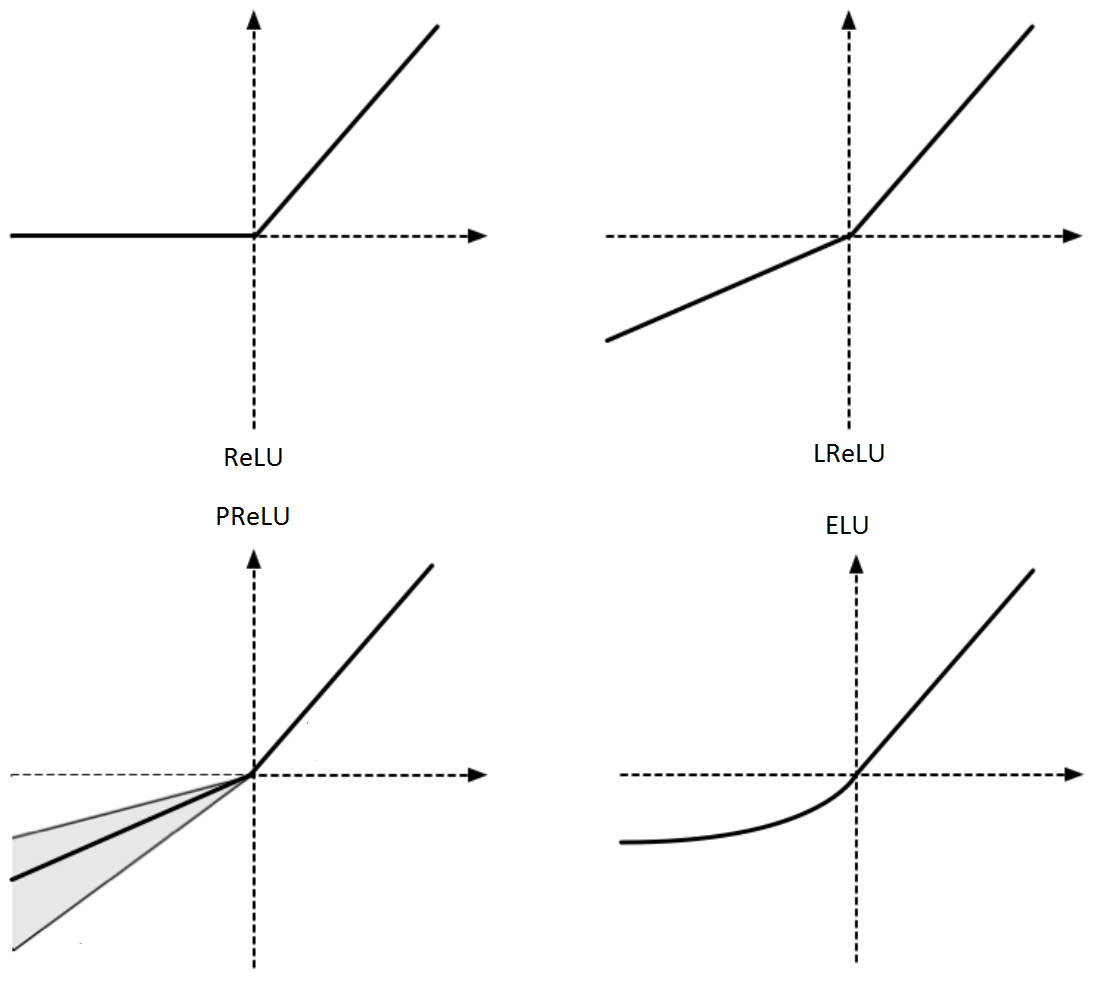
\includegraphics[width=0.85\textwidth]{figures/activations.png}
	\caption{Examples of some of the discussed activation functions. From top to bottom and left to right: ReLU, LReLU, PReLU, and ELU. \cite{}}
	\label{f:activations}
\end{figure}


\subsection{Regularization}
Some of the biggest improvements to NNs have been through regularizing the network in different ways to prevent overfitting.

\paragraph{Dropout:}
Introduced by Hinton \textit{et al.} \cite{hinton2012improving}, Dropout has shown to be very effective at improving network results and reducing overfitting. In their paper Dropout is applied to fully-connected layers where the output of the Dropout layer is 
\begin{equation}
\textbf{y} = \textbf{r} \ast a(\textbf{W}^T\textbf{x}), 
\label{eq:dropout}
\end{equation}
where $\textbf{x} = [x_1,x_2,...,x_n]^T$ is the input to the fully-connected layer, $a(\cdot)$ is an activation function, $\textbf{W}$ is the weight matrix, $\ast$ is an element-wise multiplication, and $\textbf{r}$ is a binary vector whose elements are independently drawn from a Bernoulli distribution with parameter $p$. This means that at every update to the network, each neuron has a $p$ chance of getting multiplied by zero. Dropout usually prevents the network from becoming too reliant on a few neurons and helps the network generalize by spreading feature information. Some extensions to Dropout have been proposed like in \cite{wang2013fast} where a method to improve the speed of training while using Dropout are introduced. Similar to the learned parameters of the activation functions, \cite{ba2013adaptive} learn the $p$ in the Dropout distribution adaptively. Finally, in \cite{tompson2015efficient} they modify Dropout with CNNs specifically in mind by extending the Dropout value across the entire feature map, meaning that during training each feature map has a $p$ chance of being completely ignored for each update step. They call this method Spatial Dropout and it seems to help the network learn more general features, which improves results on limited size data sets.

\paragraph{Batch Normalization:}
It is standard practice to normalize data to have zero-mean and unit variance before feeding it into a NN, but as the data goes through the network, especially deep networks, the data will lose this property. This change to the input distribution is known as internal covariance shift. To keep data normed through the network \cite{ioffe2015batch} introduced an efficient method called Batch Normalization (BN). BN works by normalizing the mean and variance of each layers input using each batch rather than the entire training set. To demonstrate BN, let $\textbf{x} = [x_1,x_2,...,x_n]^T$ be a $n$ dimensional input to a layer. The $k$-th dimensions is normalized by:
\begin{equation}
\hat{x}_k = (x_k - \mu_{B})/\sqrt{\sigma^2_B + \epsilon}
\label{eq:BN1}
\end{equation}
where $\mu_{B}$ and $\sigma^2_B$ are the mean and variance of the batch respectively and $\epsilon$ is some small constant value that will guarantee the root term is always defined. Finally the input $\hat{x}_k$ is further transformed:
\begin{equation}
y_k = \mbox{BN}_{\alpha,\beta}(x_k) = \alpha \hat{x}_k + \beta
\label{eq:BN2}
\end{equation}
where $\alpha$ and $\beta$ are parameters learned during training. There are many benefits to using BN. By reducing internal covariance shift the network will converge faster. By making sure no inputs get too large or small BN makes it possible to use saturating activation functions without fear of getting stuck in a saturating section and having vanishing gradients. This is very important when training GANs, which are extremely sensitive to the issues BN addresses.

\subsection{Architecture Improvements}
There are a couple of recent architecture improvements to NNs in general that inspired some of the newer ideas in segmentation. The first was introduced in \cite{lin2013network} where they use fully connected layers on the outputs of each convolution operation called Network-in-network. The idea was an alternative to stacking multiple convolutional layers (each with a number of their own filters) to get deepness in a neural network model, by replacing each filter with a multi-layer perceptron, which is essentially a small neural network that slides across the image like a convolutional filter. The math works out so that a $1\times 1\times U$ convolution filter convolved across a $V$-channel image emulates a $U\times V$ matrix multiplied by each $V$-channel pixel, which is the same as running a single-layer neural network across every pixel of your input as if each pixel were an example vector in a training set. Chaining together such $1\times 1\times U$ convolutions, you get the same result as if running a many-layered neural network at each input pixel of $V$ channels.  The idea from the paper was to turn a convolution filter which is a generalized linear model, into a non-linear model. It allows the network to combine channels from previous layer in a non-linear fashion, which can lead to more advanced features.

Google's team was inspired by the Network-in-network paper and saw the power of using the 1x1 convolutions not only for non-linearaity, but to reduce computational burden of deep models by using the cross-channel pooling aspect to reduce their feature maps before convolution layers. In \cite{szegedy2015going} Christian Szegedy and his team introduced the Inception module as seen in Fig.\ref{f:inceptionblock}. 

\begin{figure}[h!]
	\centering
		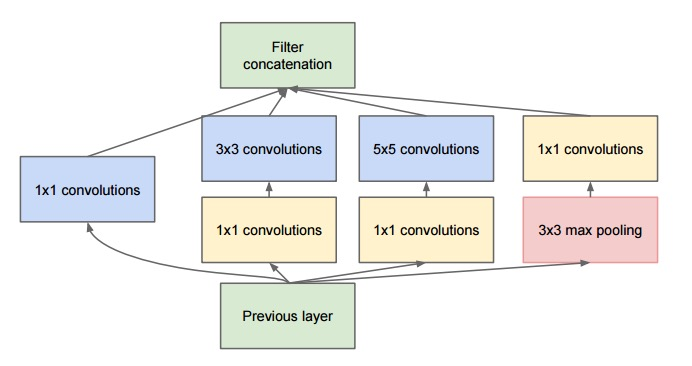
\includegraphics[width=1.0\textwidth]{figures/inceptionblock.png}
	\caption{An inception block from \cite{szegedy2015going}. Notice the 1x1 convolutions before the 3x3 and 5x5 convolutions are reducing the number of feature channels. This reduces the number of multiplications that must be performed.}
	\label{f:inceptionblock}
\end{figure}

Another work that focused on fixing the vanishing gradient problem of deep networks was Residual Nets (ResNets) \cite{he2015deep} where they used what is now called shortcut connections. These connections were inspired by Long Short Term Memory (LSTM) units, a type of recurrent neural network unit that feeds information back into itself with weighted gates. Instead of using weighted gates shortcut connections pass information with the identify function so it is untransformed. This means that the activation of deep units can be written as the sum of the activation of some shallower unit and a residual function, which is a series of network layers. Or to put simply, the input to a layer group is added to the output of that layer group. This is called a Residual Block and can be seen in Fig.\ref{f:resblock}. By stacking these residual blocks together one gets a fully residual model. This design allows the gradients to be directly propagated to shallower units allowing for networks of 100s of layers to be trained. 
\begin{figure}[h!]
	\centering
		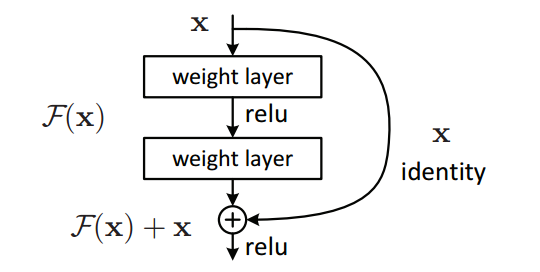
\includegraphics[width=0.80\textwidth]{figures/resblock.png}
	\caption{A residual block from \cite{he2015deep}.}
	\label{f:resblock}
\end{figure}


\section{Recent Advances in CNNs for Semantic Segmentation}\label{s:RecentAdvsCNNs}
The area of segmentation has recently seen many improvements using methods mentioned in the Section \ref{s:NNAdvances}. The highlight papers that brought big improvements to the area and that inspired the work in this thesis will be discussed each in their own section.

\subsection{Fully Convolutional Networks for Semantic Segmentation}
In \cite{long2015fully} Long \textit{et al}. used 1x1 convolutional kernels at the end of their network, instead of a fully connected layer, to produce a dense heatmap prediction of their classes as seen in Fig.~\ref{f:fcn1}. They then used \textit{backwards convolution}, sometimes called \textit{deconvolution} or \textit{transposed convolution}, with some input stride to upsample this dense heatmap back up to the original input image size. By using this method to upsample they achieve a non-linear learned upsampling. Backwards convolution works by taking the input image and padding zeros between the pixels based on the stride of the convolution shown in Fig.~\ref{f:deconv}. The result is a segmentation of classes of the same size as the input image trained fully end to end. 
\begin{figure}[h!]
	\centering
		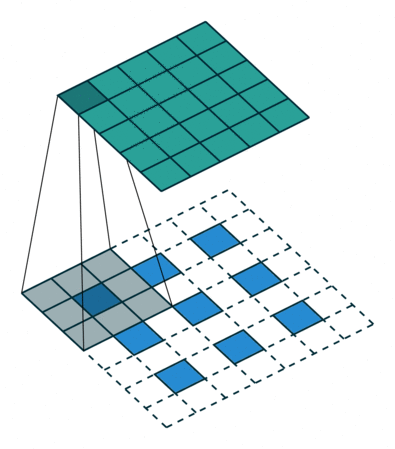
\includegraphics[width=0.50\textwidth]{figures/padding_strides_transposed.png}
	\caption{Backwards convolution with a stride of 2 upsampling a 3x3 image to a 5x5 image. Notice the 3x3 image is padded with zeros, the white tiles. The shaded grey area is the actual convolution kernel, which is learned during training.}
	\label{f:deconv}
\end{figure}
\begin{figure}[h!]
	\centering
		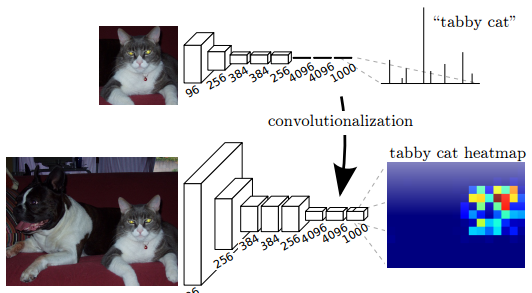
\includegraphics[width=0.90\textwidth]{figures/fcn1.png}
	\caption{Transforming fully connected layers into convolution layers enables a classification net to output a heatmap \cite{long2015fully}. This is achieved by using 1x1 convolutions instead of fully connected layers and will produce a tiny heatmap of classes. This change also make the network become independent of input image size.}
	\label{f:fcn1}
\end{figure}
However, the results are very coarse even with learned upsampling from the deconvolution layers. To remedy this they used the idea of short connections to forward information from shallow layers, upsample them to the correct matching size of the current layer, and then combine them with the current layer. This adds the finer grain detail that the shallow layers possess that get lost after pooling operations. Some of the different architectures can be seen in Fig.~\ref{f:fcn2}. Their three models used increasing number of short connections, which increased the accuracy with each additional connection. It is important to note that in this paper they used weights from a pre-trained classification network and only the new backward convolution layers and onward were learned from the segmentation maps. 
\begin{figure}[h!]
	\centering
		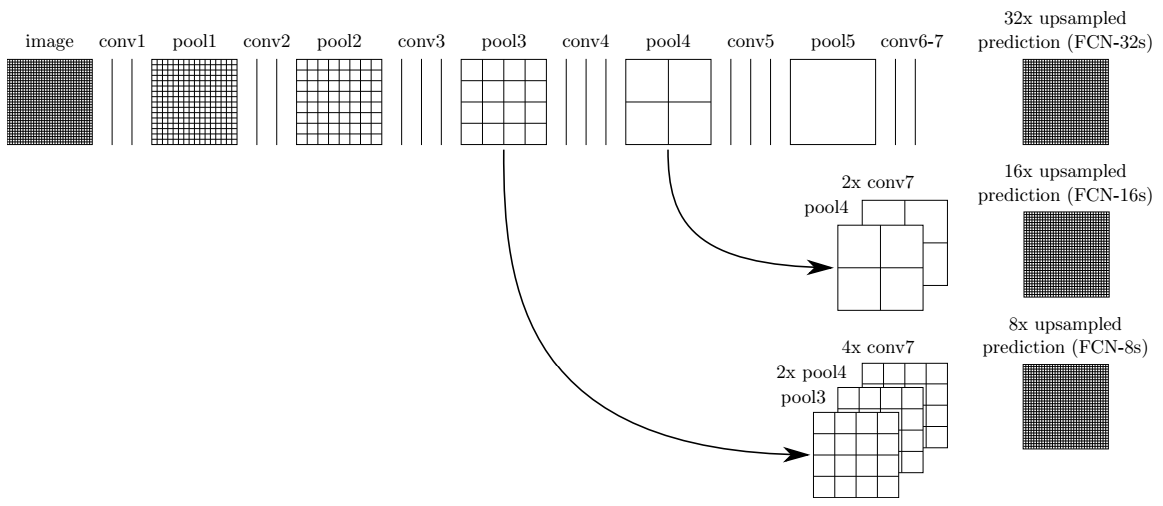
\includegraphics[width=1.0\textwidth]{figures/fcn2.png}
	\caption{Three different architectures from \cite{long2015fully}. The first uses no short connections, the second forwards information from pool4, and the third forwards information from both pool3 and pool4.}
	\label{f:fcn2}
\end{figure}

\subsection{U-Net: Convolutional Networks for Biomedical Image Segmentation}\label{s:unet}
Ronneberger \textit{et al.} in \cite{ronneberger2015u} directly mention that they are trying to improve upon results from \cite{long2015fully}. Since their application is medical segmentation the maps cannot be coarse so their aim is to improve in that area specifically as well as allowing for the network to be trained end-to-end, or no loading pre-trained weights. Their architecture consists of a contracting path (left side) into an expansive path (right side). The left side is a typical CNN and the right side is the inverse of the left, using deconvolution to upsample. Heavy use of short connections is used by forwarding information from every layer from the first half of their model to the matching size layer of the second half where it is then concatenated as shown in Fig.~\ref{f:unet}. This short connection from every layer in the contracting side differs from Long \textit{et al}., which used only two at most.
\begin{figure}[h!]
	\centering
		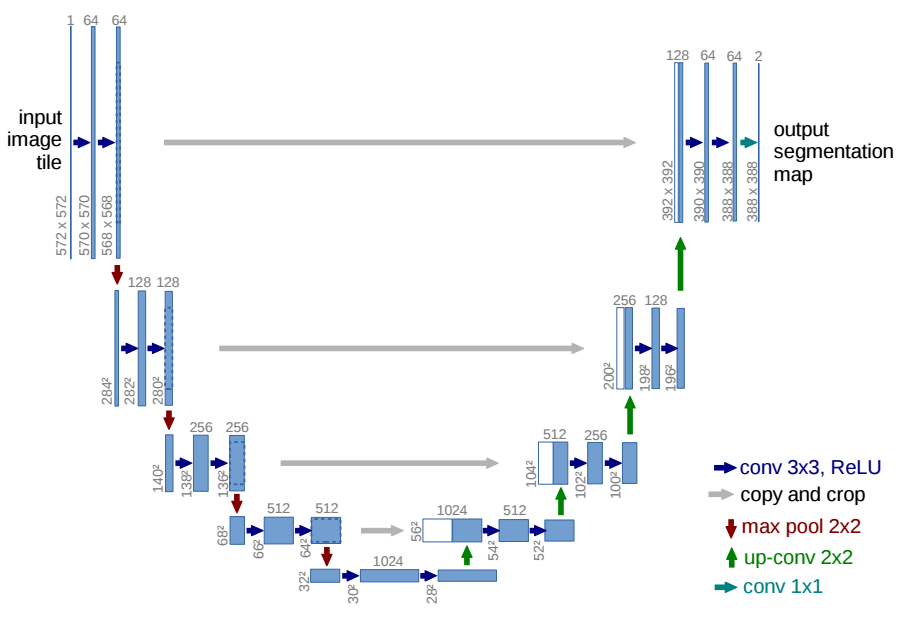
\includegraphics[width=1.0\textwidth]{figures/unet.png}
	\caption{U-Net architecture (example for 32x32 pixels in the lowest resolution). Each blue box corresponds to a multi-channel feature map. The number of channels is denoted on top of the box. The x-y-size is provided at the lower left edge of the box. White boxes represent copied feature maps. The arrows denote the different operations. \cite{ronneberger2015u}.}
	\label{f:unet}
\end{figure}
They also use an overlapping tile prediction strategy, which combats the edge artifacts from padding convolution operations with zeros. This means the prediction is only done on some middle portion of the input image.  

\subsection{Learning Iterative Processes with Recurrent Neural Networks to Correct Satellite Image Classification Maps}\label{PDERNN}
Maggiori \textit{et al.} at Inria in  \cite{maggiori2016learning} introduced a post processing network RNN whose sole purpose was to enhance segmentation results from a CNN. They formulate a generic partial differential equation (PDE) diffusion process applied to a map $u$, which is the segmentation result from the first network. They take as input a score map $u_k$ (for class $k$) and an arbitrary number of feature maps ${g_1,g_2,...,g_p}$ derived from image $I$. Then convolution kernels ${M_1,M_2,...}$ and ${N_1,N_2,...}$ are applied to the heat map $u_k$ and the features $g_j$ derived from image $I$ respectively. These filters are learned during training. These feature maps from applying these convolutions are gathered into a set:
\begin{equation}
\Phi(u_k,I) = \left\{ M_i \ast u_k, ~N_l^j \ast g_j(I);~\forall i,j,l\right\}.
\label{eq:cnnrnnset}
\end{equation}
Then $u_k$ can be expressed as changing in time as
\begin{equation}
\frac{\partial u_k(x)}{\partial t} = f_k(\Phi(u_k,I)(x)),
\label{eq:cnnrnn1}
\end{equation}
where $f_k$ is a function that takes as input the values of all the features in $\Phi(u_k,I)$ at an image point $x$ and combines them. Since it is discretized in time it takes the form:
\begin{equation}
u_{k,t+1}(x) = u_{k,t}(x) + \delta u_{k,t}(x),
\label{eq:}
\end{equation}
where $\delta u_{k,t}$ is the overall update of $u_{k,t}$ at time $t$. This $\delta u_{k,t}$ is the value that the post processing network will be trying to approximate using convolution results fed into a fully connected layer, known to be able to approximate any function, shown in Fig.\ref{f:cnnrnn1}. They do this in an iterative fashion where the update $u_{k,t+1}(x)$ is fed into the same network with shared weights $N$ number of times. They use $N = 5$ in their paper. This iterative step is a recurrent network and has a couple of advantages. First the weight sharing cuts the number of parameters down by a factor of $N$, making it easier to train. And second, the weight sharing is more physically realistic to a PDE. At each update the physics should remain unchanged, which would not be modeled properly if each iteration had a unique set of weights. An example of the complete RNN can be seen in Fig.\ref{f:cnnrnn2}.
\begin{figure}[h!]
	\centering
		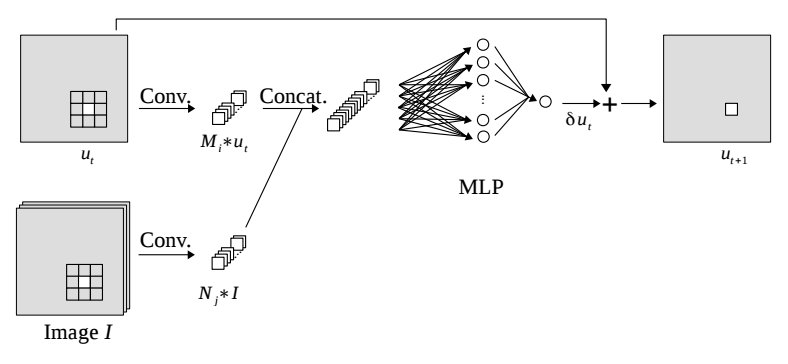
\includegraphics[width=1.0\textwidth]{figures/cnnrnn1.png}
	\caption{One iteration of the RNN represented as common neural network layers. The block approximates $\delta u_{k,t}$ and then adds it to $u_{k,t}$ to estimate $\delta u_{k,t}$. \cite{maggiori2016learning}}
	\label{f:cnnrnn1}
\end{figure}
\begin{figure}[h!]
	\centering
		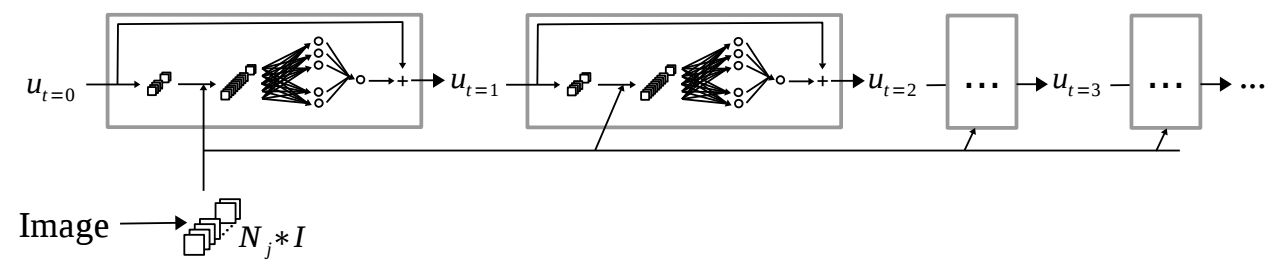
\includegraphics[width=1.0\textwidth]{figures/cnnrnn2.png}
	\caption{The whole RNN shown by multiple blocks from Fig.\ref{f:cnnrnn1} with shared weights. \cite{maggiori2016learning}.}
	\label{f:cnnrnn2}
\end{figure}


\subsection{Semantic Segmentation using Adversarial Networks}
\subsubsection{Brief overview of GANs}
We will start with a brief overview of the basics of a Generative Adversarial Network (GAN). Goodfellow \textit{et al.} introduced GANs in \cite{goodfellow2014generative} as a new way to estimate generative models, which are models that generate new data with parameters significantly smaller than the amount of data we train them on. So the models are forced to discover and efficiently internalize the essence of the data in order to generate it. 

The basic idea of GANs is to set up a game or battle between two networks. One is the generator, which creates samples that are suppose to come from the training set distribution. The other network is the discriminator, which examines an input and predicts whether it is real or fake. For example let us say our generator takes a random array of numbers sampled from a Gaussian distribution and from that array produces an image. The discriminator takes in the image and does a binary classification of either real or fake, that is, to indicate whether it is from the generator distribution or not. To fool the discriminator, the generator must learn to create images that are indistinguishable from an image from the training set.

Let us write our two networks as two functions, each of which is differentiable with respect to its own inputs and respect to its own parameters. The discriminator is a function $D$ that takes $x$ as input and uses $\theta^D$ as parameters. The generator is a function $G$ that takes $z$ as input and uses $\theta^G$ as parameters. Each network has its own cost function that it seeks to minimize. The discriminator wants to minimize $J^D(\theta^D,\theta^G)$, but must do so while only controlling $\theta^D$. Likewise, the generator wants to minimize $J^G(\theta^D,\theta^G)$, but must do so while only controlling $\theta^G$. The solution to this coupled loss system is a Nash equilibrium \cite{ratliff2013characterization}. In this context a Nash equilibrium is a tuple $(\theta^D,\theta^G)$ that is a local minimum of $J^D$ with respect to $\theta^D$ and a local minimum of $J^G$ with respect to $\theta^G$.

GANs are notoriously hard to train and much work has been done on stabilizing training. The training process involves simultaneous minimization updates to each network. On each update two batches are sampled: a batch of $x$ values from the training set and a batch of $z$ values drawn from the generator. Then two gradient steps are made simultaneously: one updating $\theta^D$ to reduce $J^D$ and the other updating $\theta^G$ to reduce $J^G$. 

After the first GAN paper many people began working on the issue of training stability and trying to produce larger, more realistic images. The first major work released was Radford \textit{et al.} \cite{radford2015unsupervised} that showed some significant improvements. They saw that using Batch Normalization in both the discriminator and generator is a must, having any fully connected layers is a bad idea, and instead of pooling use a strided convolution.

The next big improvement came from Salimans \textit{et al.} \cite{salimans2016improved} where they did slight modifications to the learning procedure. Instead of having the generator trying to fool the discriminator, they proposed a new objective function. This objective requires the generator to generate data that matches the statistics of the real data. Then the discriminator is only used to specify which statistics are worth matching. They also showed that smoothing the training labels by making the discriminator target output from [0=fake image, 1=real image] to [0=fake image, 0.9=real image] improved training stability. Their modifications focused on the loss function of the GAN, which we will see in the next two papers is a large area for improvement.

Recently some new papers have come out showing using different loss functions can greatly improve training stability and results. The first is Arjovsky \textit{et al.} \cite{arjovsky2017wasserstein} where they use the Wasserstein distance instead of the typical Kullback-Leibler divergence. Unlike Kullback-Leibler divergence, which is not defined if they generator's learned distribution and the true distribution do not overlap well, the Wasserstein distance has a well defined gradient everywhere. The second is Mao \textit{et al.} \cite{mao2017lsgan} where they reformulate the discriminator's loss as a least squares loss. The binary loss typically used does not provide more weight from a sample right next to the decision boundary to a sample very far away from the boundary. Meaning that samples that barely pass the boundary are treated the same as samples that did very well. By using the least square loss they fix this issue.

\subsubsection{GANs for segmentation}
One major issue of using CNNs for segmentation is that spatial contiguity is typically lacking, meaning that the CNN does not use long range information when classifying a pixel. We have shown some ways to combat the issue above like forwarding information from earlier layers to later layers and in Section~\ref{PDERNN} where a RNN model is run on the CNNs results to improve boundary sharpness. Luc \textit{et al.} \cite{luc2016semantic} tackled this issue by formulating the segmentation task in a way that a GAN model could be trained to accomplish as shown in Fig.~\ref{f:seggan}. Their model consists of the segmentor, which is the generator in the typical GAN framework, and the adversarial network is the discriminator. The segmentor takes an image and produces a segmentation of class predictions. The discriminator is then fed the same image and either the actual ground truth segmentation label or the segmentor's segmentation. It then predicts if the segmentation is the ground truth label or the segmentor's result. By using a GAN they combine the conventional cross-entropy loss over each pixel with an adversarial term. The adversarial term encourages the segmentation model, which is the generator, to produce label maps that cannot be distinguished from the ground-truth labels of the training set by the discriminator. Since the adversarial model can assess the joint configuration of many label variables, it can enforce forms of higher-order consistency that cannot be enforced using pair-wise terms, nor measured by a per-pixel cross-entropy loss.

\begin{figure}[h!]
	\centering
		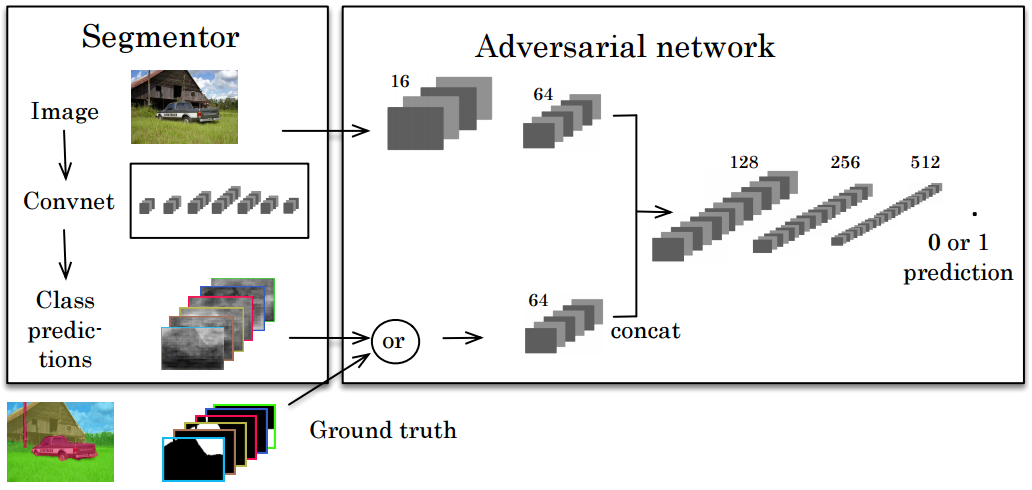
\includegraphics[width=1.0\textwidth]{figures/seggan.png}
	\caption{GAN formulation of semantic segmentation from \cite{luc2016semantic}. Left: segmentation net takes RGB image as input, and produces per-pixel class predictions. Right: Adversarial net takes label map as input and produces class label (1=ground truth, or 0=synthetic).}
	\label{f:seggan}
\end{figure}


\section{Open Questions}
There have been so many individual contributions to segmentation in the past couple of years, but combining these improvements into mixing architectures has not been studied. We intend to explore different combinations of good architectures to see if state-of-the-art can be improved. By creating the best mixed architecture we will not only have a better stand alone segmentation model, but we can hopefully further improve those results by both using it as a generator of a GAN model with untested loss functions for GAN segmentation and applying the iterative RNN process to the resulting segmentation heatmaps.
